\documentclass[../main.tex]{subfiles}
\begin{document}
\setchapterstyle{kao}
\setchapterpreamble[u]{\margintoc}
\setchapterimage[6.5cm]{Images/symmqft.jpg}
\chapter[Symmetries in Quantum Field Theory]{Symmetries in Quantum Field Theory\footnotemark[0]}
\labch{symmqft}
\section{The \href{https://en.wikipedia.org/wiki/Eugene_Wigner}{Wigner}-\href{https://en.wikipedia.org/wiki/Hermann_Weyl}{Weyl} Realization}
In Quantum Mechanics, physical states are \textbf{rays} of a \href{https://en.wikipedia.org/wiki/David_Hilbert}{Hilbert} space.\\
$\pazocal{R}=\{e^{i\lambda}\ket{\alpha};\lambda\in\mathbb{R}\}$. A space of rays is called the \textbf{projective Hilbert space}, not a vector space. The Wigner-Weyl symmetry realization is a transformation of rays into rays that leaves the transition probabilities constant:
\[
g:\pazocal{R}\to\pazocal{R}' \;\text{such that}\;p(\pazocal{R}_1\to\pazocal{R}_2)=p(\pazocal{R}'_1\to\pazocal{R}'_2)
\]
Instead of working with rays, it is easier to work with the states $\ket{\alpha}$: $g:\ket{\alpha}\to U(g)\ket{\alpha}$. The transition probability must stay the same by definition, so that we have:
\[
|(\alpha_1,\alpha_2)|=|(\alpha'_1,\alpha'_2)|=|(U\alpha_1,U\alpha_2)|
\]
There is a nice theorem by Wigner which tells us that:
\begin{theorem}[Wigner]
Symmetry transformations can be represented on the Hilbert space by either a \textbf{linear} and \textbf{unitary} operator or an \textbf{anti-linear} and \textbf{anti-unitary} operator.
\end{theorem}
Let's have a look at the two cases:
\begin{itemize}
    \item \underline{Linear and unitary}:
    \begin{enumerate}
        \item $(\alpha,U\lambda\beta)=\lambda(\alpha,U\beta)\;\lambda\in\mathbb{C}$
        \item $(\alpha,U\beta)=(U^\dagger\alpha,\beta)$
    \end{enumerate}
    \item \underline{Anti-linear and Anti-unitary}:
    \begin{enumerate}
        \item $(\alpha,U\lambda\beta)=\lambda^*(\alpha,U\beta)\;\lambda\in\mathbb{C}$
        \item $(\alpha,U\beta)=(U^\dagger\alpha,\beta)^*$
    \end{enumerate}
\end{itemize}
In both cases, we have $UU^\dagger=U^\dagger U=\mathbb{1}$. A representation of a symmetry group on a vector space $V$ is a map between elements of the group and linear operators acting on $V$ which preserves the group multiplication:
\begin{align*}
    \text{G}&\to\text{GL}(V)\xleftarrow[]{}\text{space of linear operators on $V$}\\
    g&\to r(g)\xleftarrow[]{}\text{linear operator}
\end{align*}
$r(g)$ is such that $r(g_1\cdot g_2)=r(g_1)\cdot r(g_2)$ and $r(e)=\mathbb{1}$. $g\to U(g)$ is a linear representation on the Hilbert space $\mathcal{H}$. Complications arise from the fact that representations are defined on vectors while here we are working with rays. Consider now the action of two symmetry transformations on rays:
\begin{align*}
\pazocal{R}&\xrightarrow[g_1]{}\pazocal{R}'\xrightarrow[g_2]{}\pazocal{R}''\\
\ket{\alpha}&\xrightarrow[g_1]{}U(g_1)\ket{\alpha}\xrightarrow[g_2]{}U(g_2)U(g_1)\ket{\alpha}
\end{align*}
$\ket{\alpha}\in\pazocal{R}$, $U(g_1)\ket{\alpha}\in\pazocal{R}'$ and $U(g_2)U(g_1)\ket{\alpha}\in\pazocal{R}''$ but also\\
$U(g_1\cdot g_2)\ket{\alpha}\in\pazocal{R}''$. The last one is not a requirement over the states but over the rays, so the states can differ by a phase factor and this is acceptable. \raisebox{-\mydepth}{{\includegraphics[height=1.1\baselineskip]{Images/smile.jpg}}}
\[
U(g_2)U(g_1)\ket{\alpha}=e^{i\phi_a(g_1,g_2)}U(g_1\cdot g_2)\ket{\alpha}
\]
The phase $\phi_a$ does not depend on the state $\ket{\alpha}$. To prove that, we take two linear independent states, namely $\ket{\alpha}$ and $\ket{\beta}$.
\begin{align*}
e^{i\phi_{\alpha+\beta}(g_1,g_2)}U(g_1\cdot g_2)(\ket{\alpha}+\ket{\beta})&=U(g_2)U(g_1)(\ket{\alpha}+\ket{\beta})=U(g_2)U(g_1)\ket{\alpha}+U(g_2)U(g_1)\ket{\beta}\\
&=e^{i\phi_a(g_1,g_2)}U(g_1\cdot g_2)\ket{\alpha}+e^{i\phi_\beta(g_1,g_2)}U(g_1\cdot g_2)\ket{\beta}
\end{align*}
\[
\Rightarrow e^{i\phi_{\alpha+\beta}(g_1,g_2)}(\ket{\alpha}+\ket{\beta})=e^{i\phi_a(g_1,g_2)}\ket{\alpha}+e^{i\phi_\beta(g_1,g_2)}\ket{\beta}
\]
We can now project on either $\ket{\alpha}$ or $\ket{\beta}$, being them orthogonal:\marginnote{Orthogonality comes probably from magic since we just said they are linearly independent.} 
\[
e^{\phi_{\alpha+\beta}}=e^{i\phi_\alpha}=e^{i\phi_\beta}
\]
The phase is then independent on the state, for the representation this means that we have \textbf{projective representations}:
\[
U(g_1)U(g_2)=e^{i\phi(g_1,g_2)}U(g_1\cdot g_2)
\]
Suppose to have two different classes of phases: we cannot use this rule because the phase in different classes might be different, e.g. when we treat bosons and fermions we cannot take a combination of them because they satisfy different properties (respectively, commutation and anti-commutation rules). How can we understand if the representation is projective or not? A group has an intrinsic projective representation, i.e. $\phi$ cannot be redefined if \textbf{any} of these conditions is \textbf{not} satisfied:
\begin{enumerate}
    \item The generators of the algebra can be defined in such a way that there are no \textbf{central charges} in the algebra:
    \[
    [T^a,T^b]=if^{abc}T^c+\underset{\mathclap{\tikz \node {$\uparrow$} node [below=1ex] {\footnotesize central charges };}}{C^{ab}}\mathbb{1}
    \]
    \item The group is \textbf{simply connected}.\\
    e.g. SO(3)$\sim S^3/\mathbb{Z}_2$ is a 3D sphere with equal antipodal points, it is not simply connected. The two antipodal points are the same point physically speaking, they come from the same rotation. The phase $\phi=0$ for bosonic states, while $\phi=\pm\pi$ on fermionic states. The \href{https://en.wikipedia.org/wiki/Hendrik_Lorentz}{Lorentz} group given by SO(3,1)$\sim\mathbb{R}\times S^3/\mathbb{Z}_2$ is not simply connected either.
\end{enumerate}
For every not simply connected group there exists a \textbf{universal covering} which is a simply connected group with the same algebra. In the previous examples, the universal covering of SO(3) is SU(3), the universal covering of SO(3,1) is SL$(2,\mathbb{C})$.
\subsection{Implications of Wigner-Weyl Symmetry}
Suppose now that such a representation $U(g)$ exists: the action of the symmetry transformation on the algebra of observables is \textbf{linear}. We have a state $\ket{\alpha}$: we can perform a rotation of the state without touching the reference system.
\[
\ket{\alpha}\to\ket{\alpha_g}=\bra{\alpha_g}A\ket{\alpha_g}
\]
Another possibility is to rotate the reference system without touching the state instead, $\bra{\alpha}A_{g^{-1}}\ket{\alpha}$. These two possibilities must give the same result:
\[
\ket{\alpha_g}=U(g)\ket{\alpha}\Rightarrow\bra{\alpha_g}A\ket{\alpha_g}=\bra{\alpha}U^\dagger(g)AU(g)\ket{\alpha}
\]
Hence, we can identify the transformation:
\[
A\xrightarrow[g]{}A_g=U(g)AU^\dagger(g)\quad U(g^{-1})=U^\dagger(g)
\]
Suppose to have not one, but a series of observables $A_i$ and transform them under $g$:
\[
A_i\xrightarrow[g]{}A_{ig}=U(g)A_iU^\dagger(g)=\underset{\mathclap{\tikz \node {$\uparrow$} node [below=1ex] {\footnotesize  representation of the algebra of observables};}}{R_{ij}}A_j
\]
Consider an infinitesimal transformation, we can express $R_{ij}$ as the identity+the generators of the algebra:
\[
R_{ij}(\alpha)=\delta_{ij}+it_{ij}^a\alpha^a+\pazocal{O}(\alpha^2)
\]
The same is true for the fields, $\phi_i(x)=U(g)\phi_i(x)U^\dagger(g)=R°{ij}\phi_j(x)$.\\
The charge (if it is well defined) is the \textbf{generator} of the symmetry, which means that $U(g(\alpha))=\exp{iQ^a\alpha^a}$. In the classical theory, we know that:
\[
Q^a=\int d^3xJ^{0,a}(\Vec{x},t) \quad \{Q^a,\phi_i(\Vec{x},t)\}=\frac{\partial\phi_i(\Vec{x},t)}{\partial\alpha} \quad \phi_i(x)\to\phi_i(x)+\alpha\frac{\partial\phi_i}{\partial\alpha}
\]
We want to do the same in Quantum Field Theory (QFT). Assume that there are some generators $G^a$, for an infinitesimal transformation we have:
\[
(\mathbb{1}+i\alpha^aG^a)\phi_i(x)(\mathbb{1}+i\alpha^aG^a)=\phi_i(x)+it_{ij}^a\alpha^a\phi_j(x)
\]
where we used the fact that $[G^a,\phi_i(x)]=t_{ij}^a\phi_j(x)$. In the classical theory, the charge is always well defined since the current density makes the integral convergent. However, this is generally not true in QFT, since $\pazocal{L}$ involves operator of fields in the same space-time point and this is not always well defined. For example, to regularize the integral we usually put a finite lower limit and then we send it to infinity:
\[
Q^a=\lim_{V\to\infty}\int_V d^3xJ^{0,a}(\Vec{x},t)=\lim_{V\to\infty}Q_V^a(t)
\]
where the current is defined as:
\[
J^{0,a}(x)=\frac{\delta\pazocal{L}}{\delta\Dot{\phi}_i(x)}it_{ij}^a\phi_j(x)=\pi_i(x)it_{ij}^a\phi_j(x)
\]
In the Wigner-Weyl picture, this term is well defined but it is not true in general for other symmetry realizations.\\
Another way to see that $Q^a$ is a generator is to use the properties of the generators, i.e. the structure of the algebra.\marginnote{Rivedi il conto e cerca di farlo tornare che Contino è un coglione a pedali.}
\begin{align*}
[Q^a,Q^b]&=\int d^3xd^3y[J^{0,a}(\Vec{x},t),J^{0,b}(\Vec{y},t)]\\
&=\int d^3xd^3y[\pi_i(\Vec{x},t)it_{ij}^a\phi_j(\Vec{x},t),\pi_k(\Vec{y},t)it_{kl}^b\phi_l(\Vec{y},t)]\\
&=-\int d^3xd^3y\left\{\pi_i(\Vec{x},t)t_{ij}^a[\phi_j(\Vec{x},t),\pi_k(\Vec{y},t)]t_{kl}^b\phi_l(\Vec{y},t)+\pi_k(\Vec{y},t)t_{kl}^b[\pi_i(\Vec{x},t),\phi_l(\Vec{y},t)]t_{ij}^a\phi_j(\Vec{x},t)\right\}\\
&=-\int d^3xd^3y\left[\pi_i(\Vec{x},t)t_{ij}^ai\delta_{ij}\delta^3(\Vec{x}-\Vec{y})t_{kl}^b\phi_l(\Vec{y},t)-\pi_i(\Vec{y},t)t_{kl}^bi\delta_{il}\delta^3(\Vec{x}-\Vec{y})t_{ij}^a\phi_j(\Vec{x},t)\right]\\
&=-i\int d^3x\left[\pi_i(x)t_{ij}^at_{jl}^b\phi_l(x)-\pi_k(x)t_{kl}^bt_{kl}^a\phi_j(x)\right]\\
&=-i\int d^3x\left\{\pi_i(x)[t^a,t^b]_{il}\phi_j(x)\right\}\\
&=-if^{abc}\int d^3x\pi_i(x)it_{il}^c\phi_l(x)=-if^{abc}Q^c
\marginnote[-1cm]{Rubacchio stole the plus sign and replaced it with a minus.\\
\includegraphics{Images/rubacchio.jpeg}}
\end{align*}
This is the \textbf{charge algebra}, se non ti piace vattenene a fanculo. If we work with currents instead, we obtain something similar:
\[
[J^{0,a}(\Vec{x},t),J^{0,b}(\Vec{y},t)]=if^{abc}J^{0,c}(\Vec{x},t)\delta^3(\Vec{x}-\Vec{y})
\]
At equal times, we have local properties, but in principle we could have higher order terms. There are some cases in which these terms must exist, let's look at a general case:
\[
[J^{0,a}(\Vec{x},t),J^{i,b}(\Vec{y},t)]=if^{abc}J^{i,c}(\Vec{x},t)\delta^3(\Vec{x}-\Vec{y})+S^{ab}(\Vec{x})\frac{\partial}{\partial x^i}\delta^3(\Vec{x}-\Vec{y})
\]
The extra-term is called the \href{https://en.wikipedia.org/wiki/Julian_Schwinger}{Schwinger} term. Only in particular cases we do not have higher order terms, generally for each operator with local properties at equal time we have higher order terms.

We are now trying to understand what are the consequences of the Wigner-Weyl symmetry. We have seen that the charges are the generator, we want to see what is the behaviour of the vacuum under symmetry. We are going to see that if the vacuum is \textbf{not invariant} under symmetry transformation, then the charge $Q^a$ is \textbf{not well defined} (this is called the Fabri-Picasso theorem). Consider a single charge $Q$ acting on the vacuum $\ket{0}$: we want to compute its norm.
\[
\norm{Q\ket{0}}^2=\bra{0}QQ\ket{0}=\int d^3x\bra{0}J^0(\Vec{x},t)Q\ket{0}
\]
We can use the fact that $J^0(x)=e^{-ipx}J^0(0)e^{+ipx}$:
\[
\bra{0}J^0(\Vec{x},t)Q\ket{0}=\underbrace{\bra{0}e^{-ipx}}_{\bra{0}e^{-iE_0t}}J^0(0)\underbrace{e^{+ipx}Qe^{-ipx}}_{Q}\underbrace{e^{+ipx}\ket{0}}_{e^{+iE_0t}\ket{0}}=\bra{0}J^0(0)Q\ket{0}
\]
This quantity is independent on $x$, then if we take the integral we encounter some problems:
\[
\lim_{V\to\infty}\int_Vd^3x\bra{0}J^0(0)Q\ket{0}=\infty
\]
On the other hand, if the vacuum is invariant, i.e. $Q^a\ket{0}=0$, then the physical states are classified in degenerate multiplets of the symmetry. Suppose to have a state $\ket{\alpha_i}=A_i\ket{0}$, with $A_i$ local operator which excites the vacuum. We want to show that also $A_i$ transforms as an element of the multiplet.
\[
A_i\to U(g)A_iU^\dagger(g)=R_{ij}A_j
\]
We define the state $\ket{\beta_i}$ as the action of $R_{ij}A_j$ on the vacuum $\ket{0}$.
\[
\ket{\beta_i}=R_{ij}A_j\ket{0}=U(g)A_iU^\dagger(g)\ket{0}=U(g)A_i\ket{0}=U(g)\ket{\alpha_i}
\]
Moreover, these states are \textbf{degenerate}:
\[
E_{\beta_i}=\bra{\beta_i}H\ket{\beta_i}=\bra{\alpha_i}U^\dagger(g)HU(g)\ket{\alpha_i}\underset{\mathclap{\tikz \node {$\uparrow$} node [below=1ex] {\footnotesize if $[H,U(g)]=0$ };}}{=}\bra{\alpha_i}H\ket{\alpha_i}=E_{\alpha_i}
\]
We have to prove that if the vacuum is invariant, then $[H,U(g)]=0$. This is the \href{https://en.wikipedia.org/wiki/Sidney_Coleman}{Coleman} theorem.
\begin{theorem}[Coleman]
If the vacuum is invariant, then the current is conserved.
\[
\partial_\mu J^\mu=0 \quad \text{and}\;[H,Q]=0
\]
For $Q$ well defined.
\end{theorem}
\begin{proof}
The vacuum is invariant, which means that 
\[
Q\ket{0}=\int d^3xJ^0(\Vec{x},t)\ket{0}=0
\]
We multiply on the left by a generic state $n$ with zero total momentum:
\[
\bra{n,p_n=0}J^0(\Vec{x},t)\ket{0}=\bra{n,p_n}e^{-ipx}J^0(\Vec{0},t)\underbrace{e^{+ipx}\ket{0}}_{=0}=0
\]
Consider now the derivative with respect to time of $J^0(x)$, $\bra{n,p_n=0}\partial_0J^0(x)\ket{0}$. This can be written as the total derivative of the current, since the spatial derivative is equal to zero.
\[
\bra{n,p_n=0}\Vec{\nabla}\cdot\Vec{J}(\Vec{x})\ket{0}=\bra{n,p_n=0}\Vec{\nabla}(e^{-ipx}\Vec{J}(\Vec{0)e^{+ipx}})\ket{0}=\bra{n,p_n=0}(-i\Vec{p}\Vec{j}(\Vec{x})+\Vec{J}(\Vec{x})i\Vec{p}\ket{0}=0
\]
We proved that $\bra{n,p_n=0}\partial_\mu J^\mu\ket{0}=0$. Moreover, the operator is Lorentz invariant so we can perform a boost to end up in a reference system where the momentum $p_n$ is different from zero. We have a state whose projection on all possible states is zero, this imply that:
\[
\partial_\mu J^\mu\ket{0}=0
\]
There is a nice theorem which tells us that if $O(x)\ket{0}=0$ for $O(x)$ local, then $O(x)=0$. Using this result, we have that $\partial_\mu J^\mu=0$. From this fact, we can proceed as in the classical way to prove that $dQ/dt=[H,Q]=0$.
\end{proof}
% In Quantum Electrodynamics (QED), electric charges form a multiplet of degenerate states, coming from a Wigner-Weyl symmetry. Every state has a specific electric charge (this is why $e^-$ has charge -1 and $\gamma$ has charge zero). Now we want to see this from a different point of view, using \href{https://en.wikipedia.org/wiki/George_Green_(mathematician)}{Green}'s functions. Consider the following object:
% \[
% \bra{0}T[J^{\mu,a}(x)\phi_{i_1}(x_1)\dots\phi_{i_n}(x_n)]\ket{0}
% \]
% We derive it with respect to $\partial_\mu^x$:
% \[
% \partial_\mu^x\bra{0}T[J^{\mu,a}(x)\phi_{i_1}(x_1)\dots\phi_{i_n}(x_n)]\ket{0}=\sum_{i=1}^n\bra{0}T[\phi_{i_1}(x_1)\dots\underbrace{t^a\phi(x)}_{\text{i-th term}}\dots\phi_{i_n}(x_n )]\ket{0}\delta^3(\Vec{x}-\Vec{x}_i)
% \]
% The delta comes from the derivative of the theta function inside the T-product.
\section{Approximate Symmetries and Spurion Analysis}
Spurion analysis consists basically in a fake auxiliary field which can be used to parameterize spontaneous symmetry breaking and determine all the invariant operators under that symmetry. To make things more clear, consider the case of QED:
\[
\pazocal{L}=-\frac{1}{4}F_{\mu\nu}F^{\mu\nu}+\Bar{\Psi}(i\gamma^\mu D_\mu-m)\Psi
\]
with $D_\mu=\partial_\mu-ieA_\mu$. This Lagrangian has a global U(1) symmetry and an axial U$(1)_A$ symmetry, regarding only the kinetic term:
\[
\text{U}(1):
\left\{
\begin{aligned}
&\Psi(x)\to e^{i\alpha}\Psi(x)\\
&A_\mu\to A_\mu
\end{aligned}
\right.
\quad 
\text{U}(1)_A:
\left\{
\begin{aligned}
&\Psi(x)\to e^{i\alpha\gamma_5}\Psi(x)\\
&A_\mu\to A_\mu
\end{aligned}
\right.
\]
The axial symmetry does not involve the mass term, otherwise the symmetry would be broken. To see that, let's consider a left- and a right-handed fermion defined as follows:
\[
\left\{
\begin{aligned}
&\Psi_L(x)=\frac{1-\gamma_5}{2}\Psi(x)=P_L\Psi(x)\to e^{-i\alpha}\Psi_L(x)\\
&\Psi_R(x)=\frac{1+\gamma_5}{2}\Psi(x)=P_R\Psi(x)\to e^{+i\alpha}\Psi_R(x)
\end{aligned}
\right.
\]
In the transformations we have different phases but the fields are not mixed. We now look at the mass term:
\[
m\Bar{\Psi}\Psi=m(\Bar{\Psi}_L\Psi_R+\Bar{\Psi}_R\Psi_L)\to m(e^{2i\alpha}\Bar{\Psi}_L\Psi_R+e^{-2i\alpha}\Bar{\Psi}_R\Psi_L)
\]
The mass term breaks this symmetry. To overcome the problem, consider the mass as an object which transforms:
\[
m\Bar{\Psi}\Psi\to m\Bar{\Psi}_L\Psi_R+m^*\Bar{\Psi}_R\Psi_L
\]
The spurion transformation rule tells us that $m\to e^{-2i\alpha}m$, in this way the mass term is invariant and the Lagrangian is invariant under the axial symmetry.\\
% We now want to understand how this new term behaves with this new definition.
% \[
% m\to m+\delta m \quad \text{U}(1)_A:\delta m\to e^{-2i\alpha}\delta m
% \]
% $\delta m$ must be proportional to $m$: we are \textbf{renormalizing} the mass.\marginnote{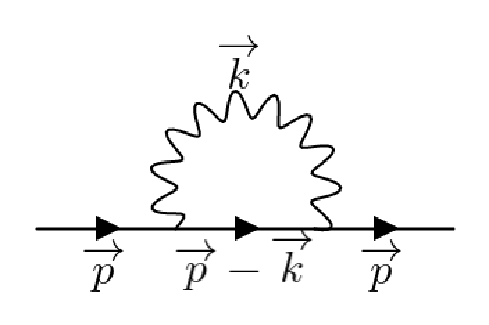
\includegraphics{Images/eselfenergy.pdf}} Naively computing the fermion propagator at first order, we expect a linear divergence for the mass, but the spurion analysis tells us that this divergence is not allowed: we have some problems with our transformations. What we can do is to send the external momentum $p$ to zero and expand around it. Doing this, we expect a logarithmically divergent term which is allowed.\\
We want to go back to the system in which the mass is real, because in order to remove the symmetry breaking we had to introduce a basis in which the mass is complex.
\[
m\Bar{\Psi}_L\Psi_R\to me^{2i\alpha}\Bar{\Psi}_L\Psi_R \quad \alpha=\pi/2: m\to-m
\]
Axial parity allows us to change the sign of the mass without symmetry breaking, but there are theories where this transformation is not allowed. Problems may arise when we have gauge invariance, where this change of sign could create additional effects, anomalies.\\
When we consider global symmetries for a theory of $N$ free fermions, we immediately encounter a complication since there are different types of fermions.
\[
\Psi=\left(\begin{array}{c}
     \xi \\
     \eta
\end{array}\right)
\begin{array}{c}
     \xleftarrow[]{}\text{left-handed field}\\
     \xleftarrow[]{}\text{right-handed field}
\end{array}
\]
Acting with the projection operators, let us easily select either the left- or the right-handed field.\marginnote{For the $\gamma$ matrices, we are working in the Weyl basis.}
\[
\gamma_5=\mqty(\dmat{-\mathbb{1},\mathbb{1}})
\quad
\Psi_L=\frac{1-\gamma_5}{2}\Psi=
\left(\begin{array}{c}
    \xi \\
     0
\end{array}\right)
\quad
\Psi_R=\frac{1+\gamma_5}{2}\Psi=
\left(\begin{array}{c}
     0 \\
     \eta
\end{array}\right)
\]
\subsection{Representations of the Lorentz Group}
The Lorentz group SO(3,1) is not compact: for non-compact groups, finite-dimensional representations are not unitary and unitary representation are infinite-dimensional. We want to understand what are the more convenient representation for $\Psi$. Our goal is to find all the finite-dimensional representations of the Lorentz group, i.e. matrices which represent the action of the group generators on the algebra. We know that SO(3,1) has an universal covering which is SL$(2,\mathbb{C})$ and we start by looking at its algebra.
\[
\forall x^\mu: X=x^\mu\sigma_\mu\left(\begin{array}{cc}
    x^0-x^3 & -x^1+ix^2 \\
    -x^1-ix^2 & x^0+x^3
\end{array}\right)
\]
where $\sigma_\mu=(\mathbb{1},-\Vec{\sigma})$ and $\det X=\norm{x}^2$. In the Lorentz group, $X$ transforms as:
\[
X\to X'=\Lambda^\mu_\nu x^\nu\sigma_\mu \quad \det X=\det X'
\]
We can also find transformations in SL$(2,\mathbb{C})$ which leaves the determinant invariant:
\[
X\to X'=AXA^\dagger \quad A\in\text{SL}(2,\mathbb{C}) \; \det X'=\det X|\det A|^2=\det X
\]
We can show that there is a map between elements of SO(3,1), i.e. $\Lambda$, and elements of SL$(2,\mathbb{C})$, i.e. $A$.
\[
\Lambda^\mu_\nu x^\nu\sigma_\mu\to Ax^\mu\sigma_\mu A^\dagger
\]
In SL$(2,\mathbb{C})$, there are two elements which correspond to $\Lambda$, which are $A$ and $-A$. We therefore have the double of the elements of SO(3,1), so the correct relations between the two groups is SO(3,1)=SL$(2,\mathbb{C})/\mathbb{Z}_2$.\\
We can define the generators of the group, corresponding to rotations $J_i$+boost $K_i$ with the following algebra:
\[
\left\{
\begin{aligned}
&[J_i,J_j]=i\epsilon_{ijk}J_k\\
&[J_i,K_j]=i\epsilon_{ijk}K_k\\
&[K_i,K_j]=i\epsilon_{ijk}J_k
\end{aligned}
\right.
\]
We can have a more convenient algebra by using combinations of generators, such as $J_i^\pm=(J_i\pm iK_i)/2$:
\[
\left\{
\begin{aligned}
&[J_i^+,J_j^+]=i\epsilon_{ijk}J^+_k\\
&[J_i^-,J_j^-]=i\epsilon_{ijk}J_k^-\\
&[J_i^+,J_j^-]=0
\end{aligned}
\right.
\Rightarrow
\mathfrak{so}(3,1)\sim\mathfrak{sl}(2,\mathbb{C})\sim\mathfrak{su}(2)\oplus\mathfrak{su}(2)
\]
Representations of $\mathfrak{su}(2)$ are the one with spin $n$ half-integer and dimension $2n+1$, representations of $\mathfrak{su}(2)\oplus\mathfrak{su}(2)$ have spin $n,m$ half integers and dimension $(2n+1)(2m+1)$. The simplest ones are (1/2,0) and (0,1/2).
\[
\left\{
\begin{aligned}
&(1/2,0): J_i^-=\sigma_i/2\; J_i^+=0\to K_i=i\sigma_i/2 \quad \text{left-handed}\\
&(0,1/2): J_i^-=0\; J_i^+=\sigma_i/2\to K_i=-i\sigma_i/2 \quad \text{right-handed}
\end{aligned}
\right.
\]
These two representations correspond exactly to Weyl fermions, a \href{https://en.wikipedia.org/wiki/Paul_Dirac}{Dirac} fermion is made as $(\frac{1}{2},0)\oplus(0,\frac{1}{2})$, a reducible representation made as the sum of two irreducible representations.\\
% How do Weyl fermions transform under the Lorentz group?
% \[
% \left\{
% \begin{aligned}
% &(1/2,0): \exp{i\alpha_iJ_i+i\beta_iK_i}=\exp{i\alpha_i\sigma_i/2-\beta_i\sigma_i/2}\\
% &(0,1/2): \exp{i\alpha_iJ_i+i\beta_iK_i}=\exp{i\alpha_i\sigma_i/2+\beta_i\sigma_i/2}
% \end{aligned}
% \right.
% \]
% We want to see if the kinetic term is invariant under this transformation:\marginnote{\[
% \gamma^0=\left(\begin{array}{cc}
%     0 & \mathbb{1} \\
%     \mathbb{1} & 0
% \end{array}\right)
% \quad
% \gamma^\mu=\left(\begin{array}{cc}
%     0 & \sigma^\mu \\
%     \Bar{\sigma}^\mu & 0
% \end{array}\right)
% \]}
% \begin{align*}
% \Bar{\Psi}i\gamma_\mu\partial_\mu\Psi&=\Psi^\dagger\gamma^0\gamma^\mu i\partial_\mu\Psi=\left(\begin{array}{cc}
%     \xi^\dagger & \eta^\dagger
% \end{array}\right)\mqty(\dmat{\Bar{\sigma}^\mu,\sigma^\mu})i\partial_\mu\left(\begin{array}{c}
%      \xi \\
%      \eta
% \end{array}\right)\\
% &=\xi^\dagger i\Bar{\sigma}^\mu\partial_\mu\xi+\eta^\dagger i\sigma^\mu\partial_\mu\eta
% \end{align*}
% where $\sigma^\mu=(\mathbb{1},\sigma^i)$ and $\bar{\sigma}^\mu=(\mathbb{1},-\sigma^i)$. For the mass term instead we have:
% \[
% \Bar{\Psi}\Psi=\Psi^\dagger\gamma^0\Psi=\left(\begin{array}{cc}
%     \xi^\dagger & \eta^\dagger
% \end{array}\right)\left(\begin{array}{cc}
%     0 & \mathbb{1} \\
%     \mathbb{1} & 0
% \end{array}\right)\left(\begin{array}{c}
%      \xi \\
%      \eta
% \end{array}\right)=\xi^\dagger\eta+\eta^\dagger\xi
% \]
The algebra $\mathfrak{sl}(2,\mathbb{C})$ is obtained by complexifying $\mathfrak{su}(2)$. For $\mathfrak{su}(2)\oplus\mathfrak{su}(2)$ we have 6 generators which can be written as $\{\sigma^i,i\sigma^i\}$, $\mathfrak{sl}(2,\mathbb{C})$ can be seen as a complex algebra with 3 generators:
\[
X=\left(\begin{array}{cc}
    0 & 1 \\
    0 & 0
\end{array}\right)
\quad
Y=\left(\begin{array}{cc}
    0 & 0 \\
    1 & 0
\end{array}\right)
\quad
H=\left(\begin{array}{cc}
    +1 & 0 \\
    0 & -1
\end{array}\right)
\]
They satisfy the following commutation rules:
\[
[X,Y]=H \quad [H,X]=2X \quad [H,Y]=-2Y
\]
Moreover, we can identify the electromagnetic field $A_\mu$ with this representation as $(\frac{1}{2},\frac{1}{2})$.
\[
\left\{
\begin{aligned}
&(0,\frac{1}{2}), (\frac{1}{2},0)=\frac{1}{2}\times0=0\times\frac{1}{2}=\frac{1}{2}\;\text{spin for both}\\
&(\frac{1}{2},\frac{1}{2})=\frac{1}{2}\times\frac{1}{2}=0+1\quad\text{4 degrees of freedom for $A_\mu$}
\end{aligned}
\right.
\]
In general, we have $(n,m)=n+m\oplus n+m-1\oplus\dots\oplus|n-m|$. For $(n,n)$ this corresponds to a traceless and symmetric tensor with rank $2n$.
\subsection{Global Symmetries}
Consider now a theory with $N$ free left-handed Weyl fermions called $\chi_i$ which transform as $(\frac{1}{2},0)$. Our goal is to write the most generic Lagrangian for this fermions:
\[
\pazocal{L}=\chi_i^\dagger i\bar{\sigma}^\mu\partial_\mu \delta_{ij}\chi_j-\frac{1}{2}(\chi_i M_{ij}\chi_j+\chi_i^\dagger(M)_{ij}^\dagger\chi_j^\dagger)
\]
The $\delta_{ij}$ comes from the diagonalization of $K_{ij}$, we can diagonalize also the mass term which is symmetric but complex, so we obtain a term $\delta_{ij}M_i$. If $M$ had not been symmetric, the mass term would have turned out to be equal to zero. The diagonalization of $M$ can be realized by a unitary transformation $U$:\marginnote{This is called the \href{https://en.wikipedia.org/wiki/Matrix_decomposition#Takagi's_factorization}{Takagi} decomposition.}
\[
M\to U^\dagger MU
\]
We want to understand what is the global symmetry which leaves the Lagrangian invariant and there are two cases:
\begin{enumerate}
    \item $M_i$ are all different, G=$(\mathbb{Z}_2)^N$. We cannot do any transformation since $U^T(\delta_{ij}M_i)U\neq\delta_{ij}M_i$. There are no continue symmetries but only a discrete one:
    \[
    P_i:
    \left\{
    \begin{aligned}
    &\chi_i\to-\chi_i\\
    &\chi_j\to\chi_j
    \end{aligned}
    \quad
    \text{for}\,i\neq j
    \right.
    \]
    \item $M\prop\mathbb{1}$, i.e. $M_{ij}=M\delta_{ij}$. If all the masses are equal, then G=O$(N)$
\end{enumerate}
Suppose now that $N=2$ (which corresponds to the case of QED), the mass term contains the two Weyl states:
\[
M=\left(\begin{array}{cc}
    0 & m \\
    m & 0
\end{array}\right)
\xrightarrow[\text{mass term}]{}
m(\chi_1\chi_2+\chi_2\chi_1+\text{h.c.})
\]
A U(1) transformation on $\chi_1$ and $\chi_2$ of the type:
\[
\left\{
\begin{aligned}
&\chi_1\to e^{+i\alpha}\chi_1\\
&\chi_2\to e^{-i\alpha}\chi_2
\end{aligned}
\right.
\]
is a symmetry sine the diagonal terms are zero. In QED, we have transformations on $\xi$ and $\eta$, which we can write using charge conjugation.
\[
\left\{
\begin{aligned}
&\text{L:}\,\xi\to e^{-i\alpha}\xi\\
&\text{R:}\,\eta\to e^{+i\alpha}\eta \quad \eta^c\to e^{-i\alpha}\eta^c
\end{aligned}
\right.
\]
If we have only a single field, the only thing we can do is $\chi\to e^{i\alpha}\chi$ but this would break the symmetry: the \href{https://en.wikipedia.org/wiki/Ettore_Majorana}{Majorana} mass term requires more fields. The only possibility if we want a gauge symmetry is that $\chi$ transforms as a real representation $r$ of the group, otherwise the mass term would not be gauge invariant.
\begin{example}
Consider now the case of $N$ free Dirac fermions:
\[
\pazocal{L}=\bar{\Psi}_L^ii\slashed{\partial}\delta_{ij}\Psi_L^j+\bar{\Psi}_R^ii\slashed{\partial}\delta_{ij}\Psi_R^j-(\bar{\Psi}_L^im_{ij}\Psi_R^i+\bar{\Psi}_R^i(m)_{ij}^\dagger\Psi_L^i)
\]
The kinetic term is symmetric under\\
U$(N)_L\times$U$(N)_R\sim$SU$(N)_L\times$SU$(N)_R\times$U$(1)_L\times$U$(1)_R$\marginnote{U$(N)=$SU$(N)\times$U$(1)/\mathbb{Z}_N$}. The center of a group G is the set of elements that commute with any other element of the group, for SU$(N)$ the center is $\mathbb{Z}_N$ which is the n-th root of the identity $e^{2\pi ki/N}$ with $k=0,1,\dots,N-1$. Let's see what is the vectorial subgroup for the symmetry group of the kinetic term.\marginnote{The vectorial subgroup is the largest subgroup which is unbroken when provided with the requirements that all the fermions are massive.}
\[
m\to U_L^\dagger mU_R:
\left\{
\begin{aligned}
&mm^\dagger\to U_L^\dagger(mm^\dagger)U_L\\
&m^\dagger m\to U_R^\dagger(m^\dagger m)U_R
\end{aligned}
\right.
\]
We choose $U_L$ and $U_R$ such that they diagonalize the last two transformations, so that $m\to U_L^\dagger mU_R=m_{diag}$.\\
If $m$ is \textbf{real} and \textbf{diagonal}, we can write the mass term as $\bar{\Psi}_im_{ij}\Psi_j$ and perform the following transformation:
\[
\left\{
\begin{aligned}
&\Psi_L^i\to e^{i\alpha_i}\Psi_L^i\\
&\Psi_R^i\to e^{i\alpha_i}\Psi_R^i
\end{aligned}
\quad\forall i=1,\dots,N
\right.
\]
The vectorial subgroup is given by [U$(1)_V$]$^N$.\\
If all the $m_i$ are \textbf{equal}, i.e. $m_{ij}=m\delta_{ij}$, then we have:
\[
\left\{
\begin{aligned}
&\Psi_L^i\to U_{ij}\Psi_L^i\\
&\Psi_R^i\to U_{ij}\Psi_R^i
\end{aligned}
\right.
\]
Now the vectorial subgroup is SU$(N)_V$. In this case, the mass term will be
\[
m\bar{\Psi}_L\mathbb{1}\Psi_R\to m\bar{\Psi}_LU^\dagger\mathbb{1}U\Psi_R=m\bar{\Psi}_L\mathbb{1}\Psi_R
\]
\end{example}
In the previous example, we saw the invariance of the kinetic term, now we can define U$(1)_V\times$U$(1)_A=$U$(1)_L\times$U$(1)_R$ where V stands for vectorial, A for axial, V=L+R and A=L-R. 
\[
\text{U}(1)_V:
\left\{
\begin{aligned}
&\Psi_L^i\to e^{i\alpha}\Psi_L^i\\
&\Psi_R^i\to e^{i\alpha}\Psi_R^i
\end{aligned}
\right.
\quad
\text{U}(1)_A:
\left\{
\begin{aligned}
&\Psi_L^i\to e^{-i\alpha}\Psi_L^i\\
&\Psi_R^i\to e^{i\alpha}\Psi_R^i
\end{aligned}
\right.
\]
The axial symmetry is a problematic one and it brings down some anomalies. We look at its generators and we will now show that they do not have a closed algebra, hence they do not form a subgroup. 
\[
T_L^a=T^a\frac{1-\gamma_5}{2} \quad T_R^a=T^a\frac{1+\gamma_5}{2}
\]
It follows from this that $T_A^a=T^a\gamma_5$ and $T_V^a=T^a$, now we compute the commutator:
\begin{align*}
[T_A^a,T_A^b]&=[T^a\gamma_5,T^b\gamma_5]=[T^a,T^b]=if^{abc}T^c=if^{abc}T_V^c
\end{align*}
The mass term breaks the symmetry, so we perform some spurion analysis.
\[
\bar{\Psi}_L^im_{ij}\Psi_R^j+\text{h.c.}\xrightarrow[]{\text{SU}(N)_L\times\text{SU}(N)_R}\bar{\Psi}_LU^\dagger_LmU_R\Psi_R+\text{h.c.}
\]
The spurionic transformation rule tells us that $m\to U_LmU^\dagger_R$, $m=(\Box,\bar{\Box})$ of SU$(N)_L\times$SU$(N)_R$.\marginnote{$\Box$ and $\bar{\Box}$ denote the fundamental and the anti-fundamental representation.}
\begin{exercise}
Consider the following theory:
\[
\pazocal{L}=\bar{\Psi}(i\slashed{\partial}-m_\Psi)\Psi+\frac{1}{2}(\partial_\mu\phi)^2-V(\phi)+y\bar{\Psi}\Psi\phi
\]
with $V(\phi)=m_\phi^2\phi^2+\lambda_3\phi^3+\lambda_4\phi^4$. Try to renormalize the fermionic mass term, how $\delta m_\Psi$ depends on the parameters and what are the associated diagrams (first for $\lambda_3=0$ then for $\lambda_3\neq0$).\\
\textbf{Solution:} we have two important symmetries here, $P_A:\Psi\to\gamma_5\Psi$ and $P_\phi: \phi\to-\phi:$
\[
P_A:
\left\{
\begin{aligned}
&m_\Psi\to-m_\Psi\\
&y\to-y\\
&\lambda_3\to\lambda_3\\
&\phi\to\phi
\end{aligned}
\right.
\quad 
P_\phi:
\left\{
\begin{aligned}
&m_\Psi\to m_\Psi\\
&y\to-y\\
&\lambda_3\to-\lambda_3\\
&\Psi\to\Psi
\end{aligned}
\right.
\]
$\bullet\lambda_3=0$:\;$\delta m_\Psi$ cannot be linearly proportional to $y$ since it changes sign under $P_\phi$, it must be proportional to $y^2$. 
\marginnote[-3cm]{
    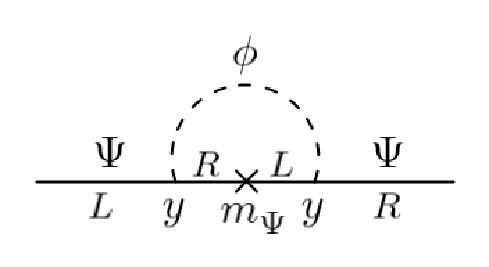
\includegraphics{Images/chiralityflip.pdf}
    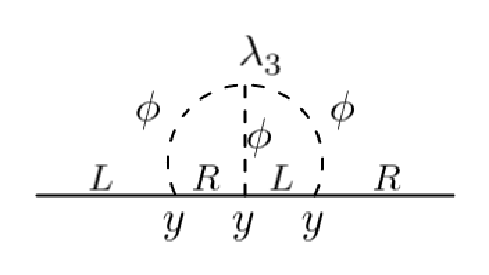
\includegraphics{Images/chiralityflip2.pdf}
    %\caption{Diagrams for $\lambda_3=0$ and $\lambda_3\neq0$.}
    }
This interaction flips the chirality.\\
$\bullet\lambda_3\neq0$:\;$\delta m_\Psi\prop\lambda_3y^3$, here we can use the \href{https://en.wikipedia.org/wiki/Hideki_Yukawa}{Yukawa} interaction to perform the chirality flip, we do not necessarily need the mass to do that.
\end{exercise}
\section{The \href{https://en.wikipedia.org/wiki/Yoichiro_Nambu}{Nambu}-\href{https://en.wikipedia.org/wiki/Jeffrey_Goldstone}{Goldstone} Realization}
Another possible way to realize symmetries is the Nambu-Goldstone realization. We know that the equations of motion can have some symmetries but their solution will not necessarily be invariant under those symmetries. We talk about Spontaneous Symmetry Breaking (SSB) when the fundamental state is not symmetric while the equations of motion are invariant under a certain symmetry. We look at the fundamental state because if it is not invariant, neither will be the excited states.\\
To make things more clear, let's take a simple example in \textbf{Classical Mechanics}: consider a rod perpendicular to a flat surface. We apply a force to it and nothing initially happens, but if we increase the force the rod will bend in some random direction: the minimal energy configuration breaks the symmetry of the equations of motion. We learnt that there is a critical value of the parameter beyond which we have SSB and that there is a manifold of degenerate vacua connected by symmetry transformations.\\
Move now to \textbf{Classical Field Theory} and consider:
\[
\pazocal{L}=\frac{1}{2}(\partial_\mu\phi)^2-\underbrace{\left(\frac{\mu^2}{2}\phi^2+\frac{\lambda}{4}\phi^4\right)}_{V(\phi)}
\]
$\phi(x)$ is a real field, we want to find the configuration which minimizes the energy. Taking $\phi(x)=$constant minimizes the kinetic energy, we have to look at the potential $V(\phi)$: for $\mu^2>0$, the system is invariant under parity $P_\phi:\phi\to\phi$ and we have no SSB. What happens if $\mu^2<0$? $V(\phi)$ has some critical points:
\[
\frac{\partial V}{\partial\phi}=0=\mu^2\phi+\lambda\phi^3\Rightarrow
\left\{
\begin{aligned}
&\phi=0\\
&\phi=\pm\sqrt{-\mu^2/\lambda}=\pm v\xleftarrow[]{}\text{vacuum expectation value (vev)}
\end{aligned}
\right.
\]
$\phi=0$ corresponds to a maximum, while we have two minima in $\phi=\pm v$: the two fundamental states are degenerate and connected by a symmetry transformation $P_\phi: \phi=+v\to\phi=-v$. The parameter in this case is $\mu^2$, the critical value is zero: for $\mu^2>0$ there is no SSB, for $\mu^2<0$ we have SSB.\\
How about SSB in \textbf{Quantum Mechanics}? Consider a particle in a double potential well $V(x)=\lambda(x^2-v^2)^2$. In this case we have tunnel effect connected to the amplitude of the maximum. Consider an Hamiltonian given by:
\[
H=\left(\begin{array}{cc}
    a & b \\
    b & a
\end{array}\right)
\]
such that $[P,H]=0$ in the subspace of the states $\ket{\pm v}$:
\[
\bra{v}H\ket{v}=a=\bra{v}P^2H\ket{v}=\bra{v}PHP\ket{v}=\bra{-v}H\ket{-v}
\]
If we have a particle confined in a well, there is a non-zero probability that after a certain time the particle will be in the other well. With similar arguments, we find:
\[
\bra{v}H\ket{-v}=\bra{-v}H\ket{v}=b
\]
After some mysterious calculations, $b$ turns out to be different from zero: this means that the eigenstates of $H$ must be combinations of $\ket{\pm v}$.
\[
\ket{\pm}=\frac{\ket{+v}\pm\ket{-v}}{2} \quad E_\pm=a\pm b
\]
Which one of these will be the fundamental state? using the nodes theorem, we see that for $b<0$ the fundamental state is $\ket{+}$ with $E_0=a+b$. Thanks to tunnel effect, we have only one fundamental state and it is no longer degenerate.\\
In \textbf{Quantum Field Theory} we can discretize the space\\
$\phi(x)\to\phi_m(x)=\phi(\Vec{x}_m,t)$, so that for each point we have a quantum mechanical variable. The tunnelling amplitude to get from $\+v$ to $-v$ will be proportional to $e^{-V}$ where $V$ is the volume of the space. Moving to continuum, the tunnelling probability goes to zero which means that if we are in a vacuum state of one of the two wells, we cannot go to the other one.\marginnote{There are some cases in QFT in which we have tunnelling but they are particular situations.} This allows us to have SSB, it is crucial to have an infinite number of variables in this situation.\\
Suppose to have a system with a large number of degrees of freedom. Realistically speaking, there will be some perturbation which gives us a small correction $\delta$ to the vacuum energy. $\delta$ is small compared to the experimental resolution but bigger than the off-diagonal terms which contribute to the tunnel effect. 
\subsection{Examples of SSB}
\begin{example}
\textbf{Ferromagnet and the \href{https://en.wikipedia.org/wiki/Ernst_Ising}{Ising} model}\\
A ferromagnet can be described as a lattice of dipoles.\marginnote{\includegraphics{Images/ising.png}}
\[
H=-\sum_{\{i,j\}}c_{ij}\Vec{\sigma}_i\cdot\Vec{\sigma}_j
\]
where the sum is extended over nearest neighbours and $c_{ij}$ are some positive valued coefficients. Such configuration depends on the temperature: for $T>T_c$, the dipoles are aligned randomly while for $T<T_c$ we have an ordered phase where all dipoles are aligned in the same direction. $H$ is invariant under SO(3) but for $T<T_c$ we have SSB, breaking SO(3)$\to$SO(2). We have an infinite number of degenerate vacuum states obtained by a rotation of a single dipole. Suppose to start in a configuration where all the dipoles are aligned in a certain direction and we want to modify. We rotate some of them, by doing this we have a cost in energy: if we want to rotate all of them, we need to use an infinite amount of energy: there will be no tunnelling.
\end{example}
\begin{example}
\textbf{Linear U(1) sigma model}\\
In Classical Field Theory, consider:
\[
\pazocal{L}=\partial_\mu\phi^\dagger\partial^\mu\phi-\underbrace{\left(\mu^2\phi^\dagger\phi+\lambda(\phi^\dagger\phi)^2\right)}_{V(\phi)}
\]
In this theory, we have a U(1) global invariance given by $\phi\to e^{i\alpha}\phi$ with $\alpha\in[0,2\pi)$. For $\mu^2>0$, we have the minimum in the origin, a non interesting situation so we consider $\mu^2<0$. Define $\varphi^2:=\phi^\dagger\phi$ and look at the critical points of $V(\phi)$:
\[
\frac{\partial V}{\partial\varphi}=2\mu^2\varphi+4\lambda\varphi^3=0\Rightarrow
\left\{
\begin{aligned}
&\varphi=0\\
&\varphi-\mu^2/2\lambda\to\varphi=v/\sqrt{2}
\end{aligned}
\right.
\]
At the minimum, we have $\phi^\dagger\phi=v^2/2$. These vacuum states are all degenerate: $\phi(x)=ve^{i\theta}/\sqrt{2}$, where $\theta$ is an arbitrary value describing the position of all the vacuum states in the manifold which are all connected by a symmetry transformation $\phi\to\phi+i\alpha\phi+\pazocal{O}(\alpha^2)$. The current associated is:
\[
J^\mu=\frac{\delta\pazocal{L}}{\delta(\partial_\mu\phi)}i\phi+\frac{\delta\pazocal{L}}{\delta(\partial\phi^\dagger)}(-i\phi^\dagger)=\partial_\mu\phi^\dagger i\phi-\partial_\mu\phi i\phi^\dagger=-i\phi^\dagger\overset{\leftrightarrow}{\partial_\mu}\phi
\]
Here it is useful to perform a change of variables and define $\phi(x)$ as:
\[
\phi(x)=\frac{e^{i\xi(x)/v}}{\sqrt{2}}(v+\eta(x)) \quad \xi(x)/v\in[0,2\pi)
\]
$\phi(x)$ is a complex field, instead of writing $\pazocal{L}$ in terms of $\mathfrak{Re}\phi$ and $\mathfrak{Im}\phi$ we use a phase and an absolute value, with the latter given by $v+\eta(x)$ and $\langle\eta(x)\rangle=0$. We compute the Lagrangian in terms of the new variables:
\[
\left\{
\begin{aligned}
&\partial_\mu\phi=i\frac{\partial_\mu\xi(x)}{v\sqrt{2}}(v+\eta(x))e^{i\xi(x)/v}+\partial_\mu\eta(x)\frac{e^{i\xi(x)/v}}{\sqrt{2}}\\
&\partial_\mu\phi^\dagger\partial^\mu\phi=\frac{1}{2}(\partial_\mu\xi(x))^2\left(1+\frac{\eta(x)}{v}\right)^2+\frac{1}{2}(\partial_\mu\eta(x))^2\\
&V(\phi)=\frac{\mu^2}{2}(v+\eta(x))^2+\frac{\lambda}{4}(v+\eta(x))^4
\end{aligned}
\right.
\]
Putting all these pieces together we get:
\begin{align*}
\pazocal{L}=&\frac{1}{2}(\partial_\mu\xi(x))^2\left(1+\frac{\eta(x)}{v}\right)^2+\frac{1}{2}(\partial_\mu\eta(x))^2\\
&-\left[\lambda v^2\eta(x)^2+\lambda v\eta(x)^3+\frac{\lambda}{4}\eta(x)^4\right]
\end{align*}
Some observations:
\begin{itemize}
    \item The field $\xi(x)$ has no potential but only the kinetic term, it represents the fluctuations around the valley of minima.
    \item The field $\eta(x)$ is massive and its interactions are not invariant under $\eta(x)\to-\eta(x)$. Can we still talk about U(1) invariance? Not with this Lagrangian but we can define a transformation rule which implements the symmetry:
    \[
    \left\{
    \begin{aligned}
    &\xi(x)\to\xi(x)+v\alpha\\
    &\eta(x)\to\eta(x)
    \end{aligned}
    \right.
    \]
    This is till a U(1) transformation, non homogeneous and in general non linear. The fields are not invariant but at the Lagrangian level symmetry is still present, we just realized it in an unusual way. At quantum level, $\xi(x)$ describes massless scalar called \textbf{Nambu-Goldstone bosons} (NGB).
    \item The manifold where $\xi(x)$ lives is the manifold of vacua ($\sim$S$^1$)
\end{itemize}
We now want to write the current in terms of $\xi(x)$ and $\eta(x)$:
\[
\left\{
\begin{aligned}
&\partial_\mu\phi=i\frac{\partial_\mu\xi(x)}{v\sqrt{2}}(v+\eta(x))e^{i\xi(x)/v}+\partial_\mu\eta(x)\frac{e^{i\xi(x)/v}}{\sqrt{2}}\\
&\phi^\dagger\partial_\mu\phi=i\frac{\partial_\mu\xi(x)}{2v}(v+\eta(x))^2+\frac{1}{2}(\partial_\mu\eta(x))(v+\eta(x))
\end{aligned}
\right.
\]
Putting everything together gives us:
\[
J^\mu=-\cancel{2}i\frac{i\partial_\mu\xi(x)}{\cancel{2}v}(v+\eta(x))^2=v\partial_\mu\xi(x)+(\text{higher orders in the fields})
\]
The current is interpolating the NGB, the U(1) symmetry has been broken into the identity.
\end{example}
\begin{example}
\textbf{O(N) linear sigma model}\\
Consider a theory of $N$ real scalar fields:
\[
\pazocal{L}=\frac{1}{2}(\partial_\mu\phi_i)(\partial^\mu\phi_i)-\underbrace{\left(\frac{\mu^2}{2}\phi_i\phi_i+\frac{\lambda}{4}(\phi_i\phi_i)^2\right)}_{V(\phi)}
\]
with $\mu^2<0$. In this case, we have a SO(N) symmetry: $\phi\to e^{iT^a\alpha^a}\phi$, $T^a\in\mathfrak{so}(N)$. The vacuum is described by $\phi(x)=\phi_0=\begin{pmatrix}0\\0\\ \vdots\\v\end{pmatrix}$ which corresponds to choosing a particular direction in the valley of minima and we can always do this since we have invariance under rotations. Conventionally, we choose coordinates so that we have $\phi_0$ in the n-th direction. Its absolute value is given by $\phi_0^T\phi_0=v^2=-\mu^2/\lambda$ and it is invariant under SO(N-1). Look now at the current $J^\mu,A$ and the charge associated $Q^A=\int d^3xJ^{0,A}(\Vec{x},t)$: does $e^{iQ^A\alpha}$ leave the vacuum invariant? The ones leaving it invariant are transformations of SO(N-1).
\begin{align*}
&\bullet \text{SO}(N-1):\; \frac{(N-1)(N-1-1)}{2} \quad \text{\# (unbroken) generators}\\
&\bullet \text{SO}(N):\;\frac{N(N-1)}{2} \quad \text{\# generators}\\
&\bullet \frac{N(N-1)}{2}-\frac{(N-1)(N-2)}{2}=N-1 \quad \text{\# broken generators}
\end{align*}
This $N-1$ broken generators are the ones which do not leave the vacuum invariant. We can write $\phi(x)$ as:
\[
\phi(x)=e^{i\xi(x)^{\hat{a}}T^{\hat{a}}/v}\begin{pmatrix}0\\0\\ \vdots\\v+\eta(x)\end{pmatrix}
\]
We want in total $N$ fields, these are given by the $N-1$ fields $\xi^{\hat{a}}(x)$+the absolute value of $\phi(x)$. The fields $\xi^{\hat{a}}(x)$ do not have a potential while $\eta(x)$ are massive and they will have interactions which do not involve derivatives. We can remove the generators that leave the vacuum invariant:
\[
iT^a=\left(
\begin{array}{cccc}
& & & 0\\
& \bigita & & \vdots\\
& & & \vdots\\
0&\dots&\dots &0\\
\end{array}
\right)
\quad
iT^{\hat{a}}=\left(
\begin{array}{ccccc}
& & & & 0\\
& &\bigzero & & \vdots\\
& & & & 1\\
& & & & \vdots\\
0&\dots& -1 &\dots &0\\
\end{array}
\right)
\]
$T^a,t^a\in\mathfrak{so}(N-1)$, we have the generators only on the $(N-1)\times(N-1)$ block above. $T^{\hat{a}}\in\mathfrak{so}(N)$ but $T^{\hat{a}}\not\in\mathfrak{so}(N-1)$, the 1 and -1 are present in the matrix above only on row $\hat{a}$ and column $\hat{a}$. SO(N) is broken into SO(N-1). It is useful to expand $\phi(x)$ at the first order in the fields:
\[
\phi(x)\simeq\left(\begin{array}{c}
     \xi^1(x)\\
     \xi^2(x)\\
     \vdots\\
     \xi^{n-1}(x)\\
     v+\eta(x)
\end{array}\right)+\text{higher orders in the fields}
\]
$\xi^{\hat{a}}(x)$ are massless and have no potential, they are excitations in the valley of minima, i.e. Goldstone bosons. We saw for the U(1) case that the current can interpolate them, we want to see it for SO(N) too.
\[
J^{\mu,A}=\frac{\delta\pazocal{L}}{\delta(\partial_\mu\phi_i)}iT_{ij}^A\phi_j=\partial_\mu\phi_iiT_{ij}^A\phi_j
\]
We want to compute the current for the broken generators.
\[
\partial_\mu\phi_i=i\frac{\partial_\mu\xi^{\hat{a}}(x)}{v}T^{\hat{a}}_{ik}\phi_k+(e^{i\xi^{\hat{a}(x)}T^{\hat{a}}/v}\phi_0)_i\frac{\partial_\mu\eta(x)}{v}
\]
When plugging this in the expression for the current, the second term disappears due to the anti-symmetry of $T_{ij}^{\hat{a}}$ so we are left with:
\[
J^{\mu,\hat{a}}=i\frac{\partial_\mu\xi^{\hat{b}}(x)}{v}T_{ik}^{\hat{b}}\phi_kiT_{ij}^{\hat{a}}\phi_j\underset{\mathclap{\tikz \node {$\uparrow$} node [below=1ex] {\footnotesize  swap $k$ and $i$, giving a - sign};}}{=}\frac{\partial_\mu\xi^{\hat{b}}(x)}{v}\overbrace{\phi_kT_{ki}^{\hat{b}}T_{ij}^{\hat{a}}\phi_j}^{\phi^TT^{\hat{b}}T^{\hat{a}}\phi}
\]
We now expand the term highlited in fancy curly brackets:
\begin{align*}
\phi^TT^{\hat{b}}T^{\hat{a}}\phi&\simeq\phi_0^TT^{\hat{b}}T^{\hat{a}}\phi_0=\phi_0^T\frac{(T^{\hat{b}}T^{\hat{a}}+T^{\hat{a}}T^{\hat{b}})}{2}\phi_0=\frac{1}{2}\phi_0^T\{T^{\hat{a}},T^{\hat{b}}\}\phi_0\\
&=\frac{1}{2}\phi_0^T2\delta_{ab}\phi_0=\phi_0^T\phi_0\delta_{ab}=v^2\delta_{ab}
\end{align*}
Which at the end of the day gives us:
\[
J^{\mu,\hat{a}}=v\partial_\mu\xi^{\hat{a}}(x)+\text{higher orders}
\]
which is exactly what we wanted to show, the broken currents interpolates the NGBs. The number of NGBs is equal to the number of broken currents, in this case (N-1). This is a general rule. As in the U(1) case, the manifold of vacua is the same as the manifold of NGBs: what is the manifold of vacua here? We have SO(N) rotations, by moving a unitary vector we have $S^{N-1}$ and the NGBs are fluctuations in this sphere with no energy cost. NGBs transform non linearly under SO(N), let's look at the transformation rules.\marginnote{A is for broken generators, V is for the unbroken generators.}
\[
\phi(x)=e^{i\xi(x)\cdot A}\left(1+\frac{\eta(x)}{v}\right)\phi_0\xrightarrow[g\in\text{SO}(N)]{}g\phi(x)=ge^{i\xi(x)\cdot A}\left(1+\frac{\eta(x)}{v}\right)
\]
We want to understand how to write the transformed NGB: any $g\in$G can be written as $g_1=e^{i\alpha\cdot A}e^{i\beta\cdot V}$ where $A\in\mathfrak{g}$ and $V\in\mathfrak{h}$, with H$\le$G.
\[
ge^{i\xi(x)\cdot A}=e^{i\xi'(\xi,g)\cdot A}e^{iu(\xi,g)\cdot V}
\]
We denoted with $\xi'(\xi,g)$ the transformed NGB.
\[
\phi'(x)=g\phi(x)=e^{i\xi'(\xi,g)\cdot A}\underbrace{e^{iu(\xi,g)\cdot V}}_{\in\text{H=SO}(N-1)}\phi_0\left(1+\frac{\eta(x)}{v}\right)
\]
The term in SO$(N-1)$ leaves the vacuum invariant by definition, hence we have:
\[
\phi'(x)=e^{i\xi'(\xi,g)\cdot A}\phi_0\left(1+\frac{\eta(x)}{v}\right)
\]
The NGB does not transform linearly, so we found two ways of realizing a symmetry: linearly (Weyl) and non-linearly (depends on the NGB).
\end{example}
\section{SSB in QFT}
At this point we want to quantize the theory and introduce the Goldstone theorem, valid also in QCD. We have already seen how to quantize the theory in the case of linearly realized symmetries: using the N\"other's theorem, we are able to compute the charge starting from the current. In the Wigner-Weyl realization we know that the current is conserved and the charge is well defined and conserved. We now want to see the case in which the charge does not annihilate the vacuum anymore, so that we cannot use Coleman's theorem and the charge will no longer be conserved. We make some assumptions:
\begin{enumerate}
    \item $S_{classical}$ is invariant under a certain symmetry
    \item $\partial_\mu J^{\mu,a}(x)=0$ as operator
    \item $Q^a\ket{0}\neq0$ for some charges.
\end{enumerate}
Suppose now to have two charges $Q^a$ and $Q^b$ which annihilate the vacuum:
\[
[Q^a,Q^b]\ket{0}=0 \quad [Q^a,Q^b]=if^{abc}Q^c
\]
The charges which annihilate the vacuum generate a linearly realized symmetry subgroup called H. For the other charges, if they do not annihilate the vacuum they are not well defined (Fabri-Picasso theorem) and the integral is not convergent.
\[
Q^a=\int d^3xJ^{0,a}(\Vec{x},t)\xrightarrow[\text{regularization}]{}Q^a_V(t)=\int_V d^3xJ^{0,a}(\Vec{x},t)
\]
The regularized version of the charge will no longer be conserved because it depends on the time, instead we can look at the commutator of the charge with a local operator $A$ located in a point $A(y)$ or located in a finite space-time region.
\[
[Q_V^a(t),A(y)]=\lim_{V\to\infty}\int_Vd^3x[J^{0,a}(\Vec{x},t),A(y)]\stackrel{?}{<}\infty
\]
For relativistic QFT, microcausality tells us that $[O_1(x),O_2(y)]=0$ for $(x-y)^2<0$, i.e. $x,y$ space-like. As $V\to\infty$, we will get $(x-y)^2<0$ so the integral will converge and the commutator of the charge with any local operator is well defined. If we fix a time such that $x$ and $y$ are space-like we must be out of the light cone, but this will eventually happen as we are integrating over $V\to\infty$. We can extend this reasoning to a local operator located in a finite space-time region by considering all the light cones centered in the points of such region and there will always be a $x$ large enough to make the integrand zero in every point of the region. We can use microcausality to prove that this commutator does not depend on time.
\begin{align*}
\frac{d}{dt}\lim_{V\to\infty}[Q_V^a(t),A]&=\lim_{V\to\infty}\int_Vd^3x\left[\frac{\partial}{\partial t}J^{0,a}(\Vec{x},t),A(y)\right]\\
&\underset{\mathclap{\tikz \node {$\uparrow$} node [below=1ex] {\footnotesize $\partial_\mu J^\mu=0$ };}}{=}\lim_{V\to\infty}\int_Vd^3x[\Vec{\nabla}\cdot\Vec{J}(\Vec{x},t),A(y)]\\
&=\lim_{V\to\infty}\int_{\partial V}dS[\hat{n}\cdot\Vec{J}(\Vec{x},t),A(y)]=0
\end{align*}
Due to microcausality, $(x-y)^2<0\;\forall x\in\partial V$. Consider now the operator $A$ to have some transformation rules under a certain symmetry:
\[
A\to U(\alpha)AU^{-1}(\alpha) \quad U(\alpha)=\exp{iQ^a\alpha^a}
\]
In our case, $Q^a$ is not well defined, we can apply this rule only in the Wigner-Weyl realization. Nevertheless we can work with the regularized version of the charge and see what happens to this transformation when sending $V\to\infty$.
\begin{align*}
\lim_{V\to\infty}U_V(\alpha)AU^{-1}_V(\alpha)&=\lim_{V\to\infty}e^{iQ_V^a\alpha^a}Ae^{-iQ_V^a\alpha^a}\\
&\simeq\lim_{V\to\infty}\left[A+i\alpha^a[Q_V^a,A]+\frac{i^2}{2}\alpha^a\alpha^b[Q_V^b,[Q_V^a,A]]+\dots\right]
\end{align*}
By defining $\delta_aA:=\lim_{V\to\infty}[Q_V^a,A]$, we can write the transformation as $A\to A+i\alpha^a\delta_aA$. The vacuum expectation value of the transformed $A$:
\[
\lim_{V\to\infty}\bra{0}U_V(\alpha)AU_V^{-1}(\alpha)\ket{0}=\lim_{V\to\infty}\bra{\alpha_V}A\ket{\alpha_V}
\]
can be seen as the limit for the transformed state $\ket{\alpha_V}$ given by\\ $\ket{\alpha_V}:=U_V^{-1}(\alpha)\ket{0}$. However, the limit of this quantity does not exist but we can overcome this problem by considering both states and taking the limit, but we cannot take the limit singularly of $\ket{\alpha_V}$. We can still consider the vacuum expectation value of some observable $A$ and the vacuum expectation value of the transformed observable $Ag^{1}$, which can be interpreted as the vacuum expectation value on the transformed state after taking the limit of $V\to\infty$. This is the expectation value of the transformed state, but we cannot directly transform it. This is because the Hilbert space must be \textbf{separable}, i.e. it must contain a countable number of basis vectors. Each vacuum state can be used to create a Hilbert space, different vacuum states contribute to different theories hence a rotation would bring our state in a space which is not the one of our theory. $Q^a\ket{0}$ is not a state on our Hilbert space, but we can still work with the expectation value of the transformed operator.
\subsection{Goldstone Theorem}
\label{GT}
The Goldstone Theorem states that for any regularized charge $Q_V^a$ such that $\lim_{V\to\infty}Q_V^a\ket{0}\neq0$ there exists a massless particle, the NGB. We give two proofs of this theorem.
\paragraph{First proof:} if $\lim_{V\to\infty}Q_V^a\ket{0}\neq0\Rightarrow\exists$ some local operator $\phi_i$ such that:
\[
\langle\delta_a\phi_i\rangle=\lim_{V\to\infty}\bra{0}[Q_V^a,\phi_i(x)]\ket{0}\neq0
\]
$\langle\delta_a\phi_i\rangle$ is called the \textbf{order parameter} and it characterizes the fact that the vacuum is not invariant. If $Q_V^a\ket{0}=0$ there cannot be an order parameter. Moreover, we have that $\frac{d}{dt}\langle\delta_a\phi_i\rangle=0$. We explicitly compute the order parameter.
\[
\langle\delta_a\phi_i\rangle=\lim_{V\to\infty}\sum_n\int_Vd^3x\left[\bra{0}J^{0,a}(\Vec{x},t)\ket{n}\bra{n}\phi_i(0)\ket{0}-\bra{0}\phi_i(0)\ket{n}\bra{n}J^{0,a}(\Vec{x},t)\ket{0}\right]
\]
Having $\phi(0)$ instead of $\phi(x)$ is just a choice we made for convenience. We know that in general we can express $J^\mu(x)$ as $e^{-iPx}J^\mu(0)e^{+iPx}$ so that the previous expression becomes:
\begin{align*}
\langle\delta_a\phi_i\rangle&=\lim_{V\to\infty}\sum_n\int_Vd^3x\left[\bra{0}e^{-iPx}J^{0,a}(0)\underbrace{e^{+iPx}\ket{n}}\bra{n}\phi_i(0)\ket{0}-\bra{0}\phi_i(0)\ket{n}\underbrace{\bra{n}e^{-iPx}}J^{0,a}(0)e^{+iPx}\ket{0}\right]\\
&=\lim_{V\to\infty}\sum_n\int_Vd^3x\left[\bra{0}J^{0,a}(0)\ket{n}\bra{n}\phi_i(0)\ket{0}e^{+iP_nx}-\bra{0}\phi_i(0)\ket{n}\bra{n}J^{0,a}(0)\ket{0}e^{-iP_nx}\right]
\end{align*}
We used the assumption that the vacuum has zero energy when applying $e^{\pm iPx}$, now we define:
\[
\int_Vd^3xe^{i\Vec{p}_n\cdot\Vec{x}}:=(2\pi)^3f_V(\Vec{p}_n)\xrightarrow[V\to\infty]{}\delta^3(\Vec{p}_n)
\]
It is possible to choose $V$ such that $f_V(\Vec{p}_n)=f_V(-\Vec{p}_n)$. For the moment, we keep the limit of finite volume and write:
\begin{align*}
\langle\delta_a\phi\rangle&=\lim_{V\to\infty}\sum_nf_V(\Vec{p}_n)\left[\bra{0}J^{0,a}(0)\ket{n}\bra{n}\phi_i(0)\ket{0}e^{iE_nt}-\bra{0}\phi_i(0)\ket{n}\bra{n}J^{0,a}(0)\ket{0}e^{-iE_nt}\right]\\
&=\sum_n\delta^3(\Vec{p}_n)\left[\bra{0}J^{0,a}(0)\ket{n}\bra{n}\phi_i(0)\ket{0}e^{iE_nt}-\bra{0}\phi_i(0)\ket{n}\bra{n}J^{0,a}(0)\ket{0}e^{-iE_nt}\right]
\end{align*}
The $\delta^3$ forces all the three-momenta to be equal to zero and the theorem states that we have massless NGBs, hence $E_n=0$ and the expression above between square brackets is different from zero.\marginnote{This last step had been revealed to me in a dream, I am 0\% sure of the correctness of this result.}\\
Once we computed the order parameter we can move to its derivative:
\[
\frac{d}{dt}\langle\delta_a\phi_i\rangle=\lim_{V\to\infty}i\sum_nf_V(\Vec{p}_n)E_n\left[\bra{0}J^{0,a}\ket{n}\bra{n}\phi_i(0)\ket{0}e^{iE_nt}+\bra{0}\phi_i(0)\ket{n}\bra{n}J^{0,a}(0)\ket{0}e^{-iE_nt}\right]=0
\]
Following the same reasoning as before, we take the limit of $V\to\infty$, $f_V(\Vec{p}_n)\to\delta^3(\Vec{p}_n)$ forces all the three-momenta to be equal to zero, resulting in $E_n=0$ since we have massless NGBs.\\
The two conditions we just proved are compatible if:
\[
\left\{
\begin{aligned}
&\bra{0}J^{0,a}\ket{n}\bra{n}\phi_i(0)\ket{0}=0\quad &&\text{for}\;E_n\neq0\\
&\bra{0}J^{0,a}\ket{n}\bra{n}\phi_i(0)\ket{0}\neq0\quad &&\text{for}\;E_n=0
\end{aligned}
\right.
\]
The last constraint is telling us that $\ket{n}$ is a massless 1-particle state. Why? Because what must be equal to zero is the product:
\[
\delta^3(\Vec{p}_n)E_n\underset{\mathclap{\tikz \node {$\uparrow$} node [below=1ex] {\footnotesize for $N$ particles };}}{=}\delta^3\left(\sum_{k=1}^N\Vec{p}_k\right)\left(\sum_{k=1}^N\sqrt{m_k^2+|\Vec{p}_k|^2}\right)
\]
The only way in which this can be zero is to have only one massless particle, $\delta^3(\Vec{p})\sqrt{m^2+|\Vec{p}|^2}=0$ when $m=0$. Let's keep only the contribution coming from massless one-particle states and see if we can obtain some more information.
\[
\langle\delta_a\phi_i\rangle=\lim_{V\to\infty}\int\frac{d^3p}{(2\pi)^3}\frac{1}{2E_p}f_V(\Vec{p})\left[\bra{0}J^{0,a}(0)\ket{\chi^b(\Vec{p})}\bra{\chi^b(\Vec{p})}\phi_i(0)\ket{0}e^{iE_nt}-\bra{0}\phi_i(0)\ket{\chi^b(\Vec{p})}\bra{\chi^b(\Vec{p})}J^{0,a}(0)\ket{0}e^{-iE_nt}\right]
\]
We want to write the matrix elements using Lorentz invariance:
\[
\bra{0}J^{\mu,a}(x)\ket{\chi^b(\Vec{p})}=iF_{ab}P^\mu e^{iPx} \quad \bra{\chi^b(\Vec{p})}\phi_i(0)\ket{0}=Z_{ab}
\]
For the first matrix element, we have to keep in mind that $\partial_\mu J^\mu=0$ so when deriving there is another factor $P^\mu$. We will have $P^2$ but since we are dealing with massless particles, the derivative of this matrix element will be equal to zero. Now we plug this in $\langle\delta_a\phi_i\rangle$:
\[
\langle\delta_a\phi_i\rangle=\lim_{V\to\infty}\int\frac{d^3p}{(2\pi)^3}\frac{1}{2\cancel{E_p}}f_V(\Vec{p})\left[iF_{ab}\cancel{E_p}Z_{ab}e^{iE_nt}+iZ_{ab}F_{ab}\cancel{E_p}e^{-iE_nt}\right]
\]
We evaluate the integral:
\[
\int\frac{d^3p}{(2\pi)^3}f_V(\Vec{p})e^{iE_nt}=1+\pazocal{O}(1/V)
\]
Similarly, for $d\langle\delta_a\phi_i\rangle/dt$ we obtain the integral:
\[
\int\frac{d^3p}{(2\pi)^3}f_V(\Vec{p})E_pe^{iE_nt}=\pazocal{O}(1/V)
\]
When taking the limit $V\to\infty$, we get
$\langle\delta_a\phi_i\rangle=iF_{ab}Z_{ab}$ while the derivative is equal to zero.\\
We expect to have an unbroken subgroup H since the symmetry is linearly realized: both $J^{\mu,a}$ and $\chi^b$ transform as some representation of the unbroken group but $J^{\mu,a}$ is interpolating $\chi^b$ from the vacuum and since they both transform as a representation of the unbroken group, this representation must be the same, being the vacuum Lorentz invariant. This explains why \# NGB=\# broken currents=\# broken generators.\\
We use the covariance under H:
\[
\bra{0}J^{\mu,a}(x)\ket{\chi^b(\Vec{p})}=\bra{0}\underbrace{U(\beta)J^{\mu,a}(x)U^{-1}(\beta)}_{\text{transformed current}}\overbrace{U(\beta)\ket{\chi^b(\Vec{p})}}^{\text{transformed state}}=R_{aa'}R_{bb'}\bra{0}J^{\mu,a'}(x)\ket{\chi^{b'}(\Vec{p})}
\]
$U(\beta)$ is a unitary operator representing the transformation, in the first step we used the fact that the vacuum is invariant under this transformation, $R_{aa'}$ is a matrix representing the current transformation, $R_{bb'}$ is a matrix for the state transformation. These two matrices must be the same since the state and the current must undergo the same transformation. This means that $F_{ab}=R_{aa'}R_{bb'}F_{a'b'}$, $F_{ab}$ is an invariant tensor under transformation of H.
\begin{example}
In SO$(N)$ the transformation $R$ is a rotation of SO$(N-1)$. Let SO$(N-1)$=H: $F_{ab}=F\delta_{ab}$, where $F$ is the decay constant of the NGB. There is only one parameter for all the NGBs, this is because of the covariance under SO$(N-1)$ so we do not need an elaborate matrix but just a number. We repeat the same argument for the other matrix element:
\[
\bra{\chi^b(\Vec{p})}\phi_i(x)\ket{0}=Z_{ib}
\]
In this example, we can choose as SO$(N-1)$ the rotations of the first $N-1$ indices: $i=1,\dots,N$ ($N$ fields) and $b=1,\dots,N-1$ ($N-1$ NGBs). Setting $i=N$ means having $Z_{Nb}=0$ because we have no vector for $N$, while $Z_{ab}=Z\delta_{ab}$ for $i=a$. We have only two quantities, $F$ and $Z$ and it is always possible to renormalize $\phi_i$ to have $Z=1$. If we now compute the order parameter we get $\langle T_{ij}^a\phi_j\rangle=iF\delta_{ia}$ where $T_{ij}^a=i(\delta_{ai}\delta_{jN}-\delta_{aj}\delta_{iN})$ are the broken generators. From this, we get $\langle\phi_j\rangle=F\delta_{jN}$ which is different from zero only for the last component, as we assumed, according with the fact that a SO$(N-1)$ rotation involves only the first $N-1$ components.
\end{example}
We proved the existence of this massless particle which must have the same quantum numbers of the current and the scalar fields. It is possible to excite the particle using both operators, which are two apparently different things but actually they are not because we have to look at transformation rules under SO$(N-1)$. $J^{\mu,a}$ transforms as the fundamental of SO$(N)$, $\phi_i(x)$ is in the fundamental of SO$(N)$ which gets broken in the fundamental of SO$(N-1)$+a singlet. Two different operators can excite the same particle, the fact that $\phi_i(x)$ is a scalar field (otherwise it would break Lorentz invariance for the vacuum) is telling us that this particle must be a boson. \marginnote{In supersymmetry theory, the field is fermionic.}\\
Goldstone theorem does not imply that these particles must be in the physical spectrum, it just states that they must exist.
\paragraph{Alternative proof:}\marginnote{St'aleternative proof fa letteralmente cagare.}
we start by computing:
\begin{align*}
\partial_\mu^x\bra{0}T[J^{\mu,a}(x)\phi_i(0)]\ket{0}&=\partial_\mu^x\left[\theta(x^0)\bra{0}J^{\mu,a}(x)\phi_i(0)\ket{0}+\theta(-x^0)\bra{0}\phi_i(0)J^{\mu,a}(x)\ket{0}\right]\\
&=\delta(x^0)\bra{0}[J^{0,a}(x),\phi_i(0)]\ket{0}
\end{align*}
Now we integrate:
\[
\int d^4x\partial_\mu^x\bra{0}T[J^{\mu,a}(x)\phi_i(0)]\ket{0}=\bra{0}[Q^a,\phi_i(0)]\ket{0}=\langle\delta_a\phi_i\rangle\neq0
\]
This is different from zero because of the presence of the massless state. We write the matrix element in \href{https://en.wikipedia.org/wiki/Joseph_Fourier}{Fourier} space.
\[
\bra{0}T[J^{\mu,a}(x)\phi_i(0)]\ket{0}=\int\frac{d^4p}{(2\pi)^4}e^{iPx}G^{\mu,a,i}(p)\xleftarrow[]{}\text{FT of the T-product, i.e. Green's function}
\]
Using Lorentz covariance, we write $G^{\mu,a,i}(p)=-iP^\mu H^{a,i}(p^2)$ and substitute it in the first integral.
\[
\int d^4pP^2\delta^4(p)H^{a,i}(p^2)
\]
If $H^{a.i}(p^2)$ has no poles the integral goes to zero, so it must be:
\[
H^{a,i}(p^2)=\frac{\langle\delta_a\phi_i\rangle}{p^2}+\text{regular terms in $p^2$}
\]
We are exciting the field in a point with the current and with $\phi_i$ in another point. The existence of the pole implies the existence of a state interpolated from the vacuum by $J^\mu$ and $\phi_i$, which propagates and gives us the pole: this is the NGB.\\

\textbf{Remarks:}
\begin{enumerate}
    \item We cannot have SSB of a symmetry (discrete or continue) in dimension $d\le2$ because of infrared divergence.
    \item How do we know if we have SSB in our theory? At the classical level, we check the derivative of the potential and look for the minima. In general, we have to look at the effective potential which includes radiative corrections, and look for the minima.
\end{enumerate}
\end{document}



%QFT beyond tree-level (QED a 1 -loop con Barducci)
%Symmetries and conservation laws (spontaneous symmetry breaking and Higgs mechanism)
%Quick intro to non-abelian gauge theories
%Effective field theories
%Intro to the SM